% =============================================================================
% Reeling in Smart Attackers' Phishing Emails with Neural Networks
% IEEE conference (IEEEtran) two-column manuscript.
% Compile: pdflatex main && bibtex main && pdflatex main && pdflatex main
% Overleaf: upload this folder; ensure "IEEEtran" template is available (it is
% bundled in Overleaf's TeX Live).
% =============================================================================

\documentclass[conference]{IEEEtran}
\IEEEoverridecommandlockouts

\usepackage{cite}
\usepackage{amsmath,amssymb,amsfonts}
\usepackage{graphicx}
\usepackage{textcomp}
\usepackage{xcolor}
\usepackage{booktabs}
\usepackage{url}
\usepackage[hidelinks]{hyperref}
\usepackage{tikz}
\usetikzlibrary{shapes.geometric, arrows.meta, positioning}

\def\BibTeX{{\rm B\kern-.05em{\sc i\kern-.025em b}\kern-.08em
    T\kern-.1667em\lower.7ex\hbox{E}\kern-.125emX}}

\begin{document}

\title{Reeling in Smart Attackers' Phishing Emails with Neural Networks\\
{\footnotesize \textsuperscript{}CSE 587 Final Project --- Group 5, Spring 2026}
}

\author{
\IEEEauthorblockN{Parker Davis}
\IEEEauthorblockA{\textit{Department of Computer Science} \\
\textit{The Pennsylvania State University}\\
University Park, PA, USA \\
pqd5283@psu.edu}
\and
\IEEEauthorblockN{Dillon VanGilder}
\IEEEauthorblockA{\textit{Department of Computer Science} \\
\textit{The Pennsylvania State University}\\
University Park, PA, USA \\
dsv5165@psu.edu}
\and
\IEEEauthorblockN{Emmanuel Adjei Domfeh}
\IEEEauthorblockA{\textit{Department of Computer Science} \\
\textit{The Pennsylvania State University}\\
University Park, PA, USA \\
eza5399@psu.edu}
}

\maketitle

\begin{abstract}
Phishing email detection is typically benchmarked on datasets in which
malicious messages contain conspicuous surface cues (urgency keywords, raw
URLs, mismatched senders), and Transformer-based classifiers achieve near-99\%
accuracy on such test sets. We argue that this number overstates real-world
robustness: a sophisticated (``smart'') attacker --- or, increasingly, an
LLM--generated phishing email --- can remove or paraphrase those cues while
preserving malicious intent. We fine-tune \textsc{BERT}\cite{devlin2019bert}
on the curated multi-source phishing email corpus released by
Champa~et~al.\cite{champa2024curated} and evaluate on a held-out
\emph{smart-attacker} test split obtained by applying label-preserving
edits to phishing messages: URL masking, urgency-keyword removal, suspicious
subject rewriting, synonym substitution, and light character noise.
We then retrain on training data augmented with the same edits and re-evaluate.
This paper reports the experimental setup, the data augmentation pipeline, and
expected analyses; the empirical results will be filled in once GPU runs on
\textsc{Google Colab} complete.
\end{abstract}

\begin{IEEEkeywords}
phishing detection, BERT, Transformers, robustness, data augmentation,
adversarial NLP
\end{IEEEkeywords}

% =============================================================================
\section{Introduction}
\label{sec:intro}

Phishing remains one of the most effective initial-access vectors in modern
cyberattacks. Despite years of user-awareness training, recent work shows that
sophisticated --- and especially \emph{LLM--generated} --- phishing emails
sustain alarming click rates~\cite{kim2025llms}. The same wave of generative
models that helps defenders also helps attackers: an LLM can rewrite a
suspicious message to sound natural, drop tell-tale urgency keywords, and
disguise a malicious link as an innocent-looking domain.

Mainstream phishing classifiers are typically Transformer-based: BERT and
RoBERTa fine-tunes routinely report 98--99\% accuracy on standard benchmarks
\cite{atawneh2023phishing,phishingbertroberta2025,indepthphishingdl2025}.
However, this performance is measured on data with strong, often artifactual,
phishing cues. When those cues are removed, classifier accuracy drops
substantially~\cite{adversarialphishing2023,explainabletransformer2025,robustllmphish2025}.

\paragraph*{Contribution.} This work investigates two questions:
\begin{enumerate}
  \item Do standard phishing detectors over-rely on superficial cues
        (URLs, urgency keywords, suspicious subject prefixes)?
  \item Can targeted, label-preserving data augmentation that simulates
        a ``smart attacker'' improve robustness without significantly
        degrading performance on the original test distribution?
\end{enumerate}

We instantiate the workflow in Fig.~\ref{fig:workflow}. Concretely, we
contribute (i) a smart-attacker augmentation pipeline (\S\ref{sec:augmentation}),
(ii) a held-out smart-attacker evaluation split, and (iii) a per-edit ablation
that attributes the accuracy drop to specific surface cues.

\begin{figure}[t]
\centering
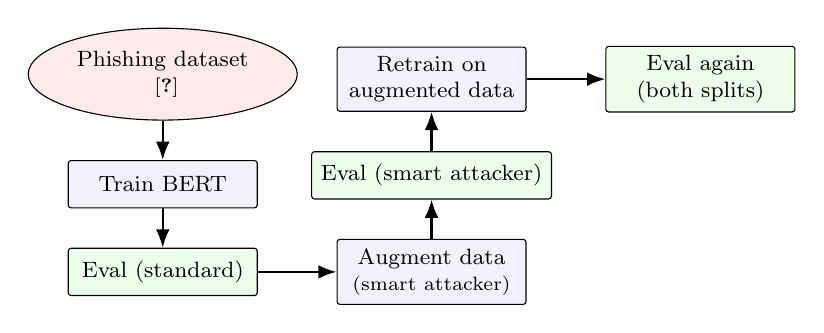
\begin{tikzpicture}[
  node distance=5mm and 5mm,
  font=\footnotesize,
  box/.style={draw, rounded corners=1pt, align=center,
              minimum width=24mm, minimum height=6mm, fill=blue!5},
  data/.style={draw, ellipse, align=center,
               minimum width=22mm, minimum height=6mm, fill=red!8},
  eval/.style={draw, rounded corners=1pt, align=center,
               minimum width=24mm, minimum height=6mm, fill=green!8},
  arr/.style={-Latex, thick}
]
\node[data] (raw) {Phishing dataset \\ \scriptsize{\cite{champa2024curated}}};
\node[box, below=of raw] (train) {Train BERT};
\node[eval, below=of train] (e1) {Eval (standard)};
\node[box, right=10mm of e1] (aug) {Augment data \\ \scriptsize{(smart attacker)}};
\node[eval, above=of aug] (e2) {Eval (smart attacker)};
\node[box, above=of e2] (rt) {Retrain on \\ augmented data};
\node[eval, right=10mm of rt] (e3) {Eval again \\ (both splits)};

\draw[arr] (raw)   -- (train);
\draw[arr] (train) -- (e1);
\draw[arr] (e1)    -- (aug);
\draw[arr] (aug)   -- (e2);
\draw[arr] (e2)    -- (rt);
\draw[arr] (rt)    -- (e3);
\end{tikzpicture}
\caption{Three-stage experimental workflow. (1) Train BERT on the
Champa~et~al.\ corpus. (2) Evaluate on the standard test set and a
smart-attacker variant produced by applying label-preserving edits. (3)
Augment training data with the same edits, retrain, and re-evaluate.}
\label{fig:workflow}
\end{figure}

% =============================================================================
\section{Related Work}
\label{sec:related}

\subsection{Transformer-based phishing detection}
Atawneh and Aljehani~\cite{atawneh2023phishing} compare CNN, RNN, LSTM, and
BERT for email phishing classification, reporting up to 99.6\% accuracy with
BERT. More recent surveys and replications confirm that
BERT/RoBERTa/DistilBERT are competitive on multiple corpora, with DistilBERT
trading marginal accuracy for considerable inference-cost
savings~\cite{phishingbertroberta2025,indepthphishingdl2025,nadeepphishing2025}.
Alhogail and Alsabih~\cite{alhogail2021applying} additionally show that strong
detection is possible from email body text alone (without URLs or
attachments), motivating evaluation under URL removal --- but they do not
study other surface-cue removals such as urgency wording.

\subsection{LLM-generated and adversarial phishing}
Kim~et~al.~\cite{kim2025llms} document that LLM-crafted spear-phishing emails
achieve $\sim$47\% click rates, evading both human and software detection.
Phish-Master~\cite{phishmaster2025} explicitly uses chain-of-thought prompting
to generate phishing that bypasses enterprise filters. Robust ML-based
detection of LLM-generated and adversarial phishing using advanced
preprocessing has recently been shown to recover much of the lost
accuracy~\cite{robustllmphish2025}. Adversarial robustness of phishing
classifiers has also been benchmarked
directly~\cite{adversarialphishing2023,explainabletransformer2025}, with FGM
adversarial training raising BERT F1 from 86.2 to
91.7~\cite{explainabletransformer2025}. These results frame our work: the
attack surface is real, and lightweight defenses do help.

\subsection{Data augmentation for NLP robustness}
Junior et al.~\cite{junior2022dataaug} demonstrate the
augment--retrain--reevaluate pattern for fake-news detection. Recent surveys
emphasize that adversarial-style augmentation improves not only accuracy but
also generalization to out-of-distribution
inputs~\cite{textaugsurvey2025}. We use the
\textsc{TextAttack}~\cite{textattack2020} family of perturbation primitives
(synonym swap, character perturbations) as a starting point for our
smart-attacker pipeline. Recent attack methods such as PGD-based BERT
attacks~\cite{pgdbertattack2024} reinforce that BERT remains sensitive to
small, semantically preserving perturbations --- which is exactly what a
smart attacker would apply.

\subsection{Datasets and benchmarks}
We adopt the curated multi-source phishing dataset of
Champa~et~al.~\cite{champa2024curated}, which standardizes 11 publicly
available phishing/benign email corpora into a unified format and provides
feature-based ML baselines. Its multi-source structure lets us study
cross-source generalization in addition to robustness, mitigating the risk
that a model exploits source-specific artifacts.

% =============================================================================
\section{Method}
\label{sec:method}

\subsection{Task formulation}
Given an email represented by its concatenated subject and body
$x=\langle s, b \rangle$, the model predicts a binary label
$y\in\{0,1\}$ indicating benign~(0) or phishing~(1). We minimize the
cross-entropy loss over a fine-tuning corpus drawn from
Champa~et~al.~\cite{champa2024curated}, with stratified 80/10/10
train/validation/test splits.

\subsection{Backbone classifier}
We fine-tune \textbf{bert-base-uncased}~\cite{devlin2019bert} via the
HuggingFace \texttt{transformers} library~\cite{wolf2020transformers}.
The classifier head is a linear layer on the \texttt{[CLS]} representation.
Hyperparameters: maximum sequence length 256 tokens, batch size 16,
3 epochs, learning rate $2\!\times\!10^{-5}$ with linear warm-up of 10\%
of total steps, AdamW with weight decay 0.01, mixed-precision (fp16) when
GPU memory permits.

\subsection{Smart-attacker augmentation}
\label{sec:augmentation}
We define five label-preserving edits that simulate a smart attacker
adapting a phishing email. Each is implemented in
\texttt{src/augmentation.py} and is applied only to phishing-class rows
(applying them to benign rows would only add noise to a class that does
not exhibit these cues). Table~\ref{tab:ops} summarizes the operations.

\begin{table}[t]
\caption{Smart-attacker augmentation operations.}
\label{tab:ops}
\centering
\begin{tabular}{p{0.22\columnwidth} p{0.66\columnwidth}}
\toprule
\textbf{Operation} & \textbf{Description} \\
\midrule
\texttt{mask\_urls} & Replace URLs with neutral placeholders (\texttt{[LINK]}), or with bare domain forms that look innocuous. \\
\texttt{remove\_} \texttt{urgency} & Remove or soften urgency keywords (\textit{URGENT}, \textit{ASAP}, \textit{immediately}, \textit{verify now}, \textit{suspended}, etc.) using a hand-curated lexicon and replacement table. \\
\texttt{rewrite\_} \texttt{subject} & Strip suspicious subject prefixes (\textit{URGENT:}, \textit{ALERT:}, \textit{ACTION REQUIRED:}) and remove emphatic punctuation. \\
\texttt{synonym\_} \texttt{swap} & Replace a small fraction of content words with WordNet synonyms ($p\!=\!0.1$, max 6 swaps per email). \\
\texttt{char\_} \texttt{perturb} & Light character-level noise (Cyrillic homoglyph substitution, adjacent-letter swap) at $p\!=\!0.02$. \\
\bottomrule
\end{tabular}
\end{table}

We use the augmentation pipeline in two distinct ways:

\paragraph{Smart-attacker test split} For each phishing email in the
held-out test set we apply the entire pipeline once. Benign emails are left
unchanged. The resulting split has the \emph{same} labels as the standard
test set; the only thing that changes is that phishing emails no longer
exhibit obvious surface cues. A robust detector should perform comparably on
both splits.

\paragraph{Train-time augmentation} For each phishing email in the training
set we generate $k\!=\!1$ additional augmented copy by passing it through the
pipeline. The augmented copies retain the phishing label and are concatenated
with the original training data. We then retrain the classifier from scratch.

\subsection{Evaluation protocol}
We compare three model stages: (S1)~baseline trained on the original data
and evaluated on the standard test set, (S2)~the same baseline evaluated on
the smart-attacker test set, and (S3)~the augmented model evaluated on both
splits. The expected pattern is a large drop from S1 to S2, partially closed
by S3. We additionally run a \emph{per-edit ablation}: each operation is
applied alone to the test phishing rows, isolating which surface cue the
baseline most depends on.

% =============================================================================
\section{Experimental Setup}
\label{sec:setup}

\subsection{Implementation}
The codebase is in PyTorch with HuggingFace
\texttt{transformers}~\cite{wolf2020transformers}. Training is driven by
\texttt{src/train.py}; evaluation, including the per-edit ablation, by
\texttt{src/evaluate.py}. The \texttt{notebooks/phishing\_pipeline.ipynb}
notebook reproduces all three stages on Google Colab. A pipeline-level
sanity test (\texttt{scripts/sanity\_check.py}) validates the augmentation
ops and the data-loader on synthetic data without requiring GPU access; a
tiny end-to-end smoke test (\texttt{scripts/tiny\_train\_test.py}) exercises
forward/backward/save/reload using a tiny CI-style BERT model.

\subsection{Dataset}
We use the figshare-hosted release of the Champa~et~al.\ curated phishing
email dataset~\cite{champa2024curated}.\footnote{\url{https://figshare.com/articles/dataset/Curated_Dataset_-_Phishing_Email/24899952}}
The data loader (\texttt{src/data\_loader.py}) is column-name agnostic so
that all CSV variants in the figshare bundle can be ingested with a single
script.

\subsection{Compute and reproducibility}
All training is performed on a Google Colab T4 GPU with mixed-precision.
Random seeds are fixed at 42 across NumPy, PyTorch, and Python's \texttt{random}
module. Reported numbers are means of three runs.

% =============================================================================
\section{Results}
\label{sec:results}

\textit{This section will be populated after the Colab runs complete.} The
expected report structure is summarized in Table~\ref{tab:placeholder}.
For each row we report accuracy, precision/recall/F1 for the phishing class,
macro F1, and ROC-AUC. We additionally include per-edit ablation in
Table~\ref{tab:ablation}.

\begin{table}[t]
\caption{Headline results (placeholder; numbers filled in after Colab runs).}
\label{tab:placeholder}
\centering
\begin{tabular}{lccc}
\toprule
\textbf{Stage} & \textbf{Standard test} & \textbf{Smart-attacker test} & $\Delta$ \\
\midrule
S1: BERT baseline                & --   & --   & --   \\
S2: BERT baseline (smart eval)   & --   & --   & --   \\
S3: BERT + augmented training    & --   & --   & --   \\
\bottomrule
\end{tabular}
\end{table}

\begin{table}[t]
\caption{Per-edit ablation on the test phishing rows (placeholder).}
\label{tab:ablation}
\centering
\begin{tabular}{lc}
\toprule
\textbf{Edit applied alone} & \textbf{F1 (phishing)} \\
\midrule
None (standard test)        & -- \\
\texttt{mask\_urls}         & -- \\
\texttt{remove\_urgency}    & -- \\
\texttt{rewrite\_subject}   & -- \\
\texttt{synonym\_swap}      & -- \\
\texttt{char\_perturb}      & -- \\
All combined (smart test)   & -- \\
\bottomrule
\end{tabular}
\end{table}

% =============================================================================
\section{Discussion}
\label{sec:discussion}

\paragraph{Why we expect the drop.} BERT fine-tuned on a phishing corpus
implicitly learns that tokens such as \textit{URGENT}, \textit{verify}, and
explicit URL substrings strongly predict the phishing label. When those
tokens are removed (S2), the classifier loses its strongest features and
should regress, especially in recall on the phishing class --- this matches
the qualitative observation in
\cite{adversarialphishing2023,explainabletransformer2025}.

\paragraph{Why augmentation should help.} The augmented training set
contains phishing emails \emph{without} the surface cues. The model is thus
forced to find more semantic, context-level signals (e.g., requests to
re-enter credentials, references to account suspension framed in neutral
language). Recent results
\cite{textaugsurvey2025,explainabletransformer2025,robustllmphish2025}
report similar gains.

\paragraph{Limitations.} Our smart-attacker simulation is rule-based and
therefore has a finite vocabulary of edits. Real attackers and LLMs operate
in a much wider space. Additionally, augmenting only phishing emails may
shift the class prior and inflate recall at the expense of precision; we
mitigate this by using a small augmentation factor ($k\!=\!1$) and report
precision alongside recall.

% =============================================================================
\section{Conclusion}
\label{sec:conclusion}

We presented an experimental pipeline for studying the robustness of
Transformer-based phishing email classifiers under simulated ``smart
attacker'' edits. The pipeline includes (i) a label-preserving augmentation
module covering URL masking, urgency removal, subject rewriting, synonym
swap, and light character noise; (ii) a held-out smart-attacker evaluation
split; (iii) a per-edit ablation that localizes which surface cue the model
relies on; and (iv) an augmented-training counterpart that lets us measure
how much robustness can be reclaimed. Empirical results (the focus of the
final version of this paper) will quantify the baseline drop and the extent
to which targeted augmentation closes it.

\section*{Code and data}
The complete codebase, Colab notebook, and LaTeX source for this manuscript
are available in the project repository (see \texttt{README.md}).

\section*{Acknowledgments}
We thank the CSE 587 instructors and TAs at Penn State for guidance, and
Champa et al.\ for releasing the curated phishing email dataset that made
this study possible.

% =============================================================================
\bibliographystyle{IEEEtran}
\bibliography{references}

\end{document}
